\section{Experiments}
\label{sec:exp}

\begin{table*}[t] \footnotesize

\begin{tabular}{|l|l|l|}
\hline
Distributional Models & \mto & \vm \\
\hline
\cite{Lamar:2010:LCU:1870658.1870736} & .708 & -\\ %algorithm name LDC
\cite{Brown:1992:CNG:176313.176316}* & .678 & .630\\
%kcls(Och,1999) & .737 & .656\\
%\cite{goldwater-griffiths:2007:ACLMain} & .632 & .562\\
(Goldwater et al., 2007) & .632 & .562\\
\cite{Ganchev:2010:PRS:1859890.1859918}* & .625 & .548\\
\cite{maron2010sphere} & .688 (.0016)&-\\
Bigrams (Sec.~\ref{sec:bigram}) & \bgmto & \bgvm \\
Partitions (Sec.~\ref{sec:rpart}) & \rpmto & \rpvm \\
Substitutes (Sec.~\ref{sec:wordsub}) & \wsmto & \wsvm \\
\hline
\end{tabular}
\begin{tabular}{|l|l|l|}
\hline
Models with Additional Features & \mto & \vm \\
\hline
\cite{Clark:2003:CDM:1067807.1067817}* & .712 & .655 \\
\cite{christodoulopoulos-goldwater-steedman:2011:EMNLP} & .728 & .661\\
\cite{bergkirkpatrick-klein:2010:ACL} & .755 & -\\ % Interesting in  christo paper:73.9/67.7
\cite{Christodoulopoulos:2010:TDU:1870658.1870714} & .761 & .688\\
\cite{blunsom-cohn:2011:ACL-HLT2011} & .775 & .697\\
Substitutes and Features (Sec.~\ref{sec:feat}) & \ftmto & \ftvm \\
& & \\
& & \\
\hline
\end{tabular}

\caption{Summary of results in terms of the \mto and \vm scores.
  Standard errors are given in parentheses when available.  Starred
  entries have been reported in the review paper
  \cite{Christodoulopoulos:2010:TDU:1870658.1870714}.  Distributional
  models use only the identity of the target word and its context.
  The models on the right incorporate orthographic and
  morphological features.}
\label{tab:results}
\end{table*}

In this section we present experiments that evaluate substitute
vectors as representations of word context within the S-CODE
framework.  Section~\ref{sec:bigram} replicates the bigram based
S-CODE results from \cite{maron2010sphere} as a baseline.  The S-CODE
algorithm works with discrete inputs.  The substitute vectors as
described in Section~\ref{sec:lm} are high dimensional and continuous.
We experimented with two approaches to use substitute vectors in a
discrete setting.  Section~\ref{sec:rpart} presents an algorithm that
partitions the high dimensional space of substitute vectors into small
neighborhoods and uses the partition id as a discrete context
representation.  Section~\ref{sec:wordsub} presents an even simpler
model which pairs each word with a random substitute.  When the
left-word -- right-word pairs used in the bigram model are replaced
with word -- partition-id or word -- substitute pairs we see
significant gains in accuracy.  These results support our running
hypothesis that paradigmatic features, i.e. potential substitutes of a
word, are better determiners of syntactic category compared to left
and right neighbors.  Section~\ref{sec:feat} explores morphologic and
orthographic features as additional sources of information and its
results improve the state-of-the-art in the field of unsupervised
syntactic category acquisition.

Each experiment was repeated 10 times with different random seeds and
the results are reported with standard errors in parentheses or error
bars in graphs.  Table~\ref{tab:results} summarizes all the results
reported in this paper and the ones we cite from the literature.

\subsection{Bigram model}\label{sec:bigram}

In \cite{maron2010sphere} adjacent word pairs (bigrams) in the corpus
are fed into the S-CODE algorithm as $X, Y$ samples.  The algorithm
uses stochastic gradient ascent to find the $\phi_x, \psi_y$
embeddings for left and right words in these bigrams on a single
25-dimensional sphere.  At the end each word $w$ in the vocabulary
ends up with two points on the sphere, a $\phi_w$ point representing
the behavior of $w$ as the left word of a bigram and a $\psi_w$ point
representing it as the right word.  The two vectors for $w$ are
concatenated to create a 50-dimensional representation at the end.
These 50-dimensional vectors are clustered using an instance weighted
k-means algorithm and the resulting groups are compared to the correct
part-of-speech tags.  Maron et al. \shortcite{maron2010sphere} report
many-to-one scores of .6880 (.0016) for 45 clusters and .7150 (.0060)
for 50 clusters (on the full PTB45 tag-set).  If only $\phi_w$ vectors
are clustered without concatenation we found the performance drops
significantly to about .62.

To make a meaningful comparison we re-ran the bigram experiments using
our default settings and obtained a many-to-one score of \bgmto\ 
and the V-measure is \bgvm\  for 45 clusters.  The following
default settings were used: (i) each word was kept with its original
capitalization, (ii) the learning rate parameters were adjusted to
$\varphi_0=50$, $\eta_0=0.2$ for faster convergence in log likelihood,
(iii) the number of s-code iterations were increased from 12 to 50
million, (iv) k-means initialization was improved using
\cite{arthur2007k}, and (v) the number of k-means restarts were
increased to 128 to improve clustering and reduce variance.

\subsection{Random partitions}\label{sec:rpart}

Instead of using left-word -- right-word pairs as inputs to S-CODE we
wanted to pair each word with a paradigmatic representation of its
context to get a direct comparison of the two context representations.
To obtain a discrete representation of the context, the
random--partitions algorithm first designates a random subset of
substitute vectors as centroids to partition the space, and then
associates each context with the partition defined by the closest
centroid in cosine distance.  Each partition thus defined gets a
unique id, and word ($X$) -- partition-id ($Y$) pairs are given to
S-CODE as input.  The algorithm cycles through the data until we get
approximately 50 million updates.  The resulting $\phi_x$ vectors are
clustered using the k-means algorithm (no vector concatenation is
necessary).  Using default settings (64K random partitions, 25 s-code
dimensions, $Z=0.166$) the many-to-one accuracy is \rpmto\ and
the V-measure is \rpvm.

To analyze the sensitivity of this result to our specific parameter
settings we ran a number of experiments where each parameter was
varied over a range of values.

\begin{figure}[ht] \centering
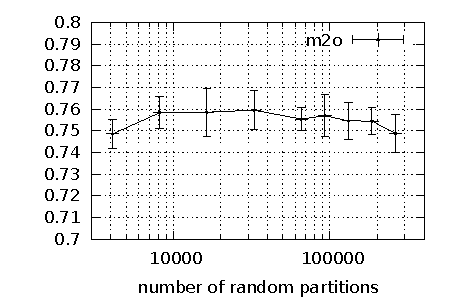
\includegraphics[width=\linewidth]{plot-p.pdf}
\caption{\mto is not sensitive to the number of partitions used to
  discretize the substitute vector space within our experimental
  range.}
\label{plot-p}
\end{figure}

Figure~\ref{plot-p} gives results where the number of initial random
partitions is varied over a large range and shows the results to be
fairly stable across two orders of magnitude.

\begin{figure}[ht] \centering
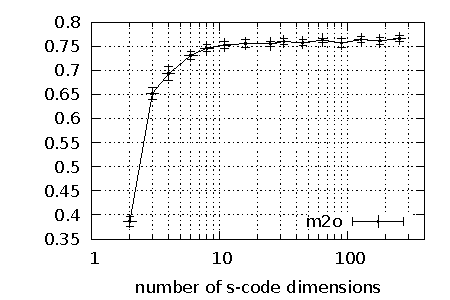
\includegraphics[width=\linewidth]{plot-d.pdf}
\caption{\mto falls sharply for less than 10 S-CODE dimensions, but
  more than 25 do not help.}
\label{plot-d}
\end{figure}

Figure~\ref{plot-d} shows that at least 10 embedding dimensions are
necessary to get within 1\% of the best result, but there is no
significant gain from using more than 25 dimensions.

\begin{figure}[ht] \centering
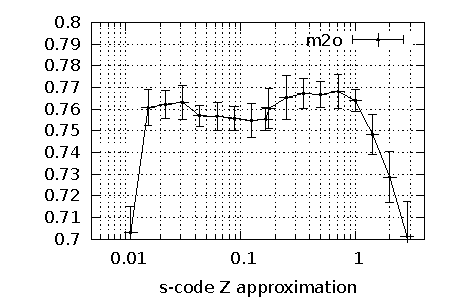
\includegraphics[width=\linewidth]{plot-z.pdf}
\caption{\mto is fairly stable as long as the $\tilde{Z}$ constant is
  within an order of magnitude of the real $Z$ value.}
\label{plot-z}
\end{figure}

Figure~\ref{plot-z} shows that the constant $\tilde{Z}$ approximation
can be varied within two orders of magnitude without a significant
performance drop in the many-to-one score.  For uniformly distributed
points on a 25 dimensional sphere, the expected $Z\approx 0.146$.  In
the experiments where we tested we found the real $Z$ always to be in
the 0.140-0.170 range.  When the constant $\tilde{Z}$ estimate is too
small the attraction in Eq.~\ref{eq:attract} dominates the repulsion
in Eq.~\ref{eq:repulse} and all points tend to converge to the same
location.  When $\tilde{Z}$ is too high, it prevents meaningful
clusters from coalescing.
%%% I have seen the first, but the second is pure guess, need to
%%% look.  The distances seem to be decreasing on that end as well!

We find the random partition algorithm to be fairly robust to different
parameter settings and the resulting many-to-one score significantly
better than the bigram baseline.

\subsection{Random substitutes}\label{sec:wordsub}

Another way to use substitute vectors in a discrete setting is simply
to sample individual substitute words from them.  The
random-substitutes algorithm cycles through the test data and pairs
each word with a random substitute picked from the pre-computed
substitute vectors (see Section~\ref{sec:lm}).  We ran the
random-substitutes algorithm to generate 14 million word ($X$) --
random-substitute ($Y$) pairs (12 substitutes for each token) as input
to S-CODE.  Clustering the resulting $\phi_x$ vectors yields a
many-to-one score of \wsmto\ and a V-measure of \wsvm.

This result is close to the previous result by the random-partition
algorithm, \rpmto, demonstrating that two very different discrete
representations of context based on paradigmatic features give
consistent results.  Both results are significantly above the bigram
baseline, \bgmto.  Figure~\ref{plot-s} illustrates that the
random-substitute result is fairly robust as long as the training
algorithm can observe more than a few random substitutes per word.

\begin{figure}[ht] \centering
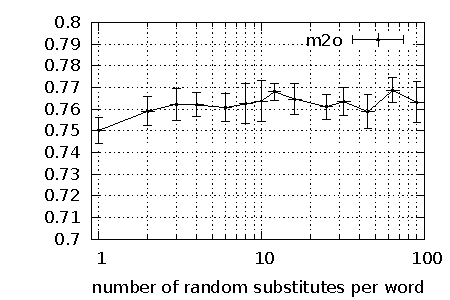
\includegraphics[width=\linewidth]{plot-s.pdf}
\caption{\mto is not sensitive to the number of random substitutes
  sampled per word token.}
\label{plot-s}
\end{figure}

\subsection{Morphological and orthographic features}\label{sec:feat}

Clark \shortcite{Clark:2003:CDM:1067807.1067817} demonstrates that
using morphological and orthographic features significantly improves
part-of-speech induction with an HMM based model.
Section~\ref{sec:related} describes a number other approaches that
show similar improvements.  This section describes one way to
integrate additional features to the random-substitute model.

%% In order to accommodate multiple feature types the CODE model needs to
%% be extended to handle more than two variables.
%% \cite{globerson2007euclidean} suggest the following likelihood
%% function:

%% \begin{eqnarray}
%% &\ell(\phi,& \psi^{(1)}, \ldots, \psi^{(K)}) = \label{eq:multicode}\\
%% &&\sum_k w_k \sum_{x,y^{(k)}} \bar{p}(x,y^{(k)}) \log p(x,y^{(k)}) \nonumber
%% \end{eqnarray}

%% \noindent where $Y^{(1)}, \ldots, Y^{(K)}$ are $K$ different variables
%% whose empirical joint distributions with $X$,
%% $\bar{p}(x,y^{(1)})\ldots\bar{p}(x,y^{(K)})$, are known.
%% Eq.~\ref{eq:multicode} then represents a set of CODE models
%% $p(x,y^{(k)})$ where each $Y^{(k)}$ has an embedding $\psi_y^{(k)}$
%% but all models share the same $\phi_x$ embedding.  The weights $w_k$
%% reflect the relative importance of each $Y^{(k)}$.

%% We adopt this likelihood function, set all $w_k=1$, let $X$
%% represent a word, $Y^{(1)}$ represent a random substitute and
%% $Y^{(2)}, \ldots, Y^{(K)}$ stand for various morphological and
%% orthographic features of the word.  With this setup, the training
%% procedure needs to change little: each time a word --
%% random-substitute pair is sampled, the relevant word -- feature pairs
%% are also generated and input to the gradient ascent algorithm.

The orthographic features we used are similar to the ones in
\cite{bergkirkpatrick-EtAl:2010:NAACLHLT} with small modifications:

\begin{itemize}
\item Initial-Capital: this feature is generated for capitalized words
  with the exception of sentence initial words.
\item Number: this feature is generated when the token starts with a
  digit.
\item Contains-Hyphen: this feature is generated for lowercase words
  with an internal hyphen.
\item Initial-Apostrophe: this feature is generated for tokens that
  start with an apostrophe.
\end{itemize}

%%% dy: which wsj?  1M?  why not 156M??
We generated morphological features using the unsupervised algorithm
Morfessor \cite{creutz05}.  Morfessor was trained on the WSJ section
of the Penn Treebank using default settings, and a perplexity
threshold of 300.  The program induced 5 suffix types that are present
in a total of 10,484 word types.  These suffixes were input to S-CODE
as morphological features whenever the associated word types were
sampled.

In order to incorporate morphological and orthographic features into
S-CODE we modified its input.  For each word -- random-substitute pair
generated as in the previous section, we added word -- feature pairs
to the input for each morphological and orthographic feature of the
word.  Words on average have 0.25 features associated with them.
This increased the number of pairs input to S-CODE from 14.1
million (12 substitutes per word) to 17.7 million (additional 0.25
features on average for each of the 14.1 million words).

Using similar training settings as the previous section, the addition
of morphological and orthographic features increased the many-to-one
score of the random-substitute model to \ftmto\ and V-measure to \ftvm.
Both these results improve the state-of-the-art in part-of-speech
induction significantly as seen in Table~\ref{tab:results}.

\begin{figure*}[ht] \centering
\vspace*{-25mm}
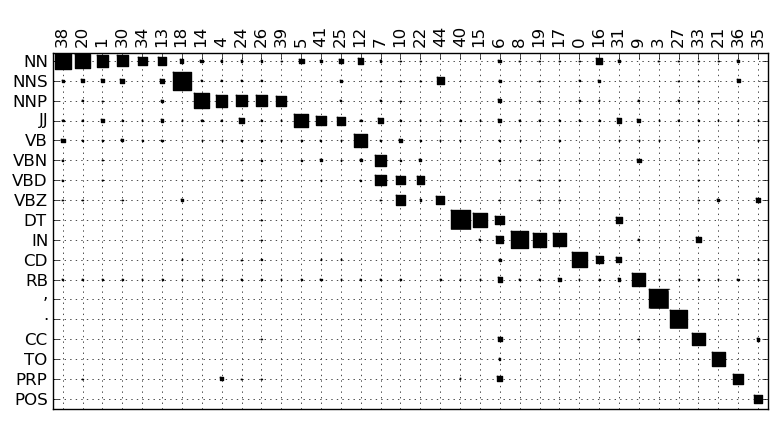
\includegraphics[width=\textwidth]{hinton.png}
\vspace*{-30mm}
\caption{Hinton diagram comparing most frequent tags and clusters.}
\label{plot-hinton}
\end{figure*}

